\label{sec:processing}
Die gefilterten EEG-Sequenzen durchlaufen nun eine Verarbeitungskette (Abb. \ref{fig:data_processing}). Im ersten Schritt werden die Signale auf das Intervall 1 bis -1 normalisiert , dazu werden die Signale durch den jeweiligen Maximalwert bzw. Betrag des Minimalwertes geteilt. Dieses Vorgehen stellt sicher, dass die absolute Amplitude keinen Einfluss auf die Gewichtung im Klassifikator hat. Zudem wird die Datenmenge wiederum reduziert. Im zweiten Schritt werden die Signale in Frequenzbänder (EEG-Bänder) unterteilt. Hierzu werden bestimmte Frequenzbereiche aus dem Signal entfernt, sodass nur die gewünschten Frequenzen erhalten bleiben. Diese EEG-Bänder gliedern sich in folgende Frequenzbereiche und werden nach griechischen Buchstaben benannt:
\begin{itemize}
 \item $\delta$ : 0,1 bis < 4Hz
 \item $\theta$ :   4 bis < 8Hz
 \item $\alpha$ :   8 bis < 13Hz
 \item $\beta$  :  13 bis < 30Hz
 \item $\gamma$ :  > 30Hz
\end{itemize}
Den Frequenzbändern werden verschiedene Eigenschaften zugesprochen. Delta Wellen treten bei Erwachsenen häufig in der traumlosen Tiefschlafphase auf. Theta-Wellen zeigen sich bei Schläfrigkeit und leichtem Schlaf. Mit leichter Entspannung und entspannter Wachheit (mit geschlossenen Augen) werden Alpha-Wellen assoziiert. Beta Wellen treten während der REM-Schlafphase oder unter Einwirkung von Psychopharmaka auf. Gamma-Wellen gehen häufig mit starker Konzentration oder Meditation einher.

Um die einzelnen Frequenzbänder zu erhalten ist eine Filterfunktion notwendig. Für die Anwendung wurde hierfür ein Buttworth-Filter\cite{Butterworth30} eingesetzt. Gleichung \ref{eq:butterworth} zeigt die Übertragungsfunktion mit $A_0$: Gleichspannungsverstärkung, $\Omega = \frac{f}{f_g}$: auf Grundfrequenz normierte Frequenz und $n$: Ordnung des Filters. Abbildung \ref{fig:butterworth_filter} zeigt exemplarisch Filterfunktionen verschiedener Ordnung mit den Grenzen von 500 bis 1250Hz. Alle Frequenzen darunter und darüber werden deutlich abgeschwächt bzw. gehen gegen null. Der Butterworth-Filter verläuft nahe Eins im gewünschten Bereich, fällt an den Grenzen ab und stellt sicher, dass das Signal an den Grenzen um $\frac{1}{\sqrt{2}} \approx 0.7071$ gemindert wird. Je höher die Ordnung, desto steiler geht die Funktion durch die angegebenen Grenzen. Der Filter lässt sich gut in Hardware realisieren.

\begin{equation} \label{eq:butterworth}
\left|\underline{A}\right|^2 = \frac{A_0^2}{1+ k_{2n} \Omega ^{2n}}
\end{equation}

\begin{figure}[h] 
  \begin{center}
    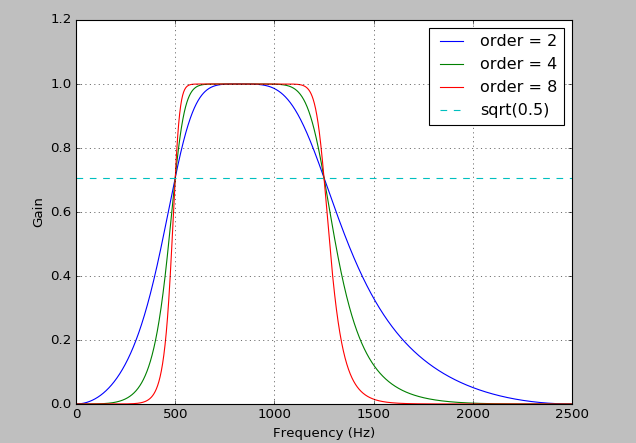
\includegraphics[width=5.5cm]{butterworth_filter}
    \caption[Butterworth-Filter]{Die Filterfunktion eines Butterworthfilters 2., 4,. und 8. Ordnung im Frequenzbereich von 500 bis 1250Hz. \label{fig:butterworth_filter}}
  \end{center}
\end{figure}